\documentclass[convert={outfile=\jobname.svg}]{standalone}

\usepackage{tikz}
\usetikzlibrary{shapes.geometric}

\begin{document}
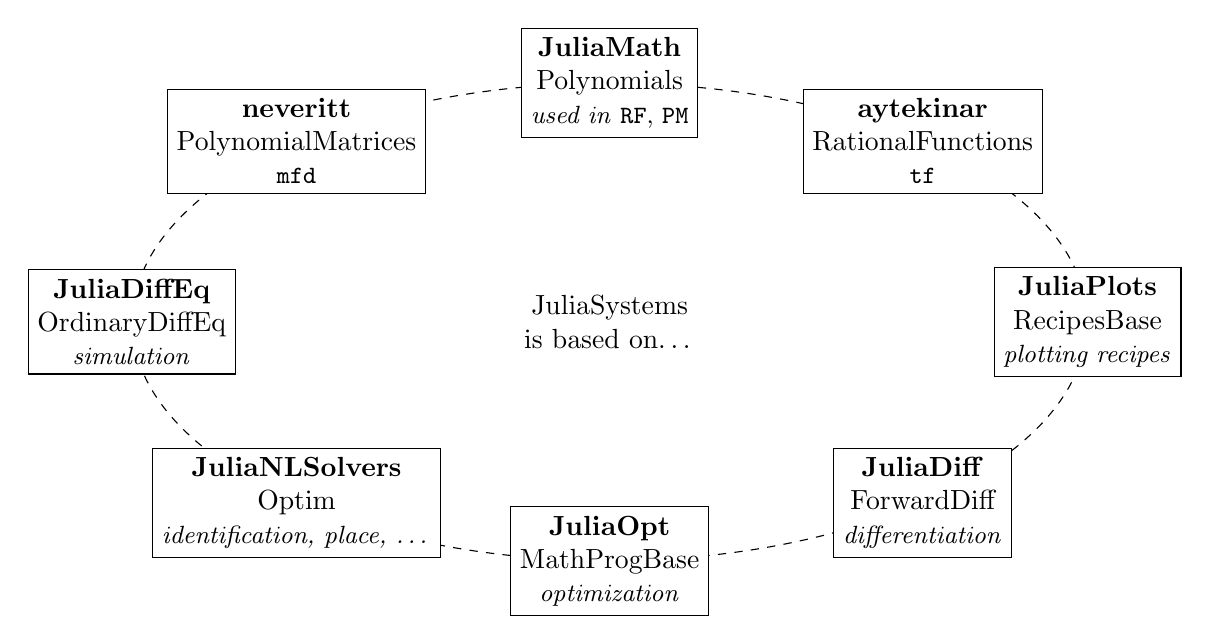
\begin{tikzpicture}
  \node [shape = ellipse, minimum width = \linewidth,
        minimum height = 0.5\linewidth, align = center, draw, dashed]
        (be) {JuliaSystems\\is based on\dots};

  \foreach \angle/\org/\pkg/\dsc [count = \id] in {
    30/aytekinar/RationalFunctions/{\texttt{tf}},
    90/JuliaMath/Polynomials/{\emph{used in} \texttt{RF}, \texttt{PM}},
    150/neveritt/PolynomialMatrices/{\texttt{mfd}},
    210/JuliaNLSolvers/Optim/{\emph{identification, place, \dots}},
    270/JuliaOpt/MathProgBase/{\emph{optimization}},
    330/JuliaDiff/ForwardDiff/{\emph{differentiation}},
    180/JuliaDiffEq/OrdinaryDiffEq/{\emph{simulation}},
    0/JuliaPlots/RecipesBase/{\emph{plotting recipes}}
  } \node [draw, shift = (be.\angle), align = center, rectangle, fill = white]
          (tb\id) {\textbf{\org}\\\pkg\\\small\dsc};
\end{tikzpicture}
\end{document}
